31. $\cfrac{(x^2+14x+49)(16-x^2)}{x^2-6x+9}\geqslant0\Leftrightarrow\cfrac{-(x+7)^2(x-4)(x+4)}{(x-3)^2}\geqslant0.$ Применив метод интервалов, найдём ответ: $x\in
\{-7\}\cup[-4;3)\cup(3;4].$
\begin{figure}[ht!]
\center{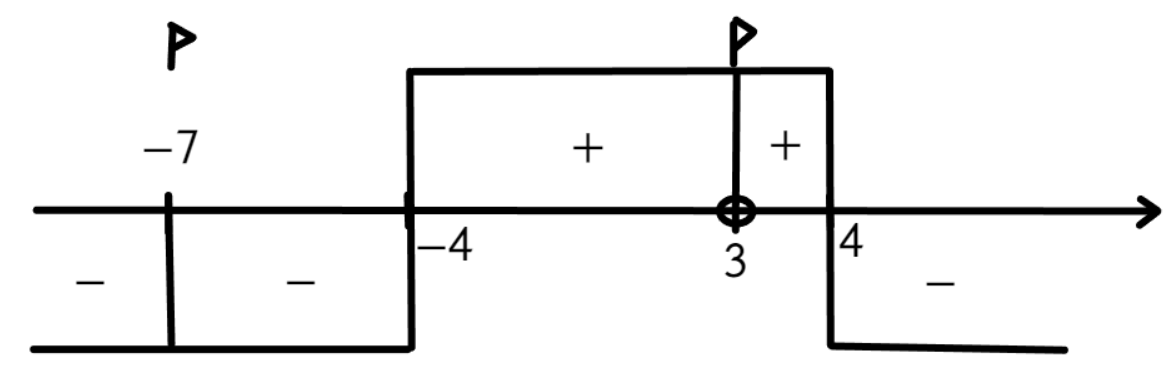
\includegraphics[scale=0.35]{ner9-31.png}}
\end{figure}\\
